\chapter{Implementace}
\label{sec:implementation}
Tato kapitola obsahuje již konkrétní popis implementace aplikace, její návrh a je zde popsáno i UI, včetně UX.
Samotná aplikace je psána celá v jednom React.js projektu a obsahuje již zmíněné technologie z kapitoly \ref{sec:technologies}.

\section{Implementace strojů}
\label{sec:machine_impl}
Aplikace obsahuje dohromady tři stroje, ze kterých je samotná simulace brána jako samostatný stroj. 
Zbylé dva stroje jsou tedy Turingův stroj a RAM stroj.

Všechny stroje jsou reprezentovány třídou, která dědí ze třídy \texttt{Machine}. Ta definuje různé sjednocené operace
pro všechny stroje, jako je například funkce \texttt{reset}, \texttt{backstep} a nebo \texttt{restoreState}. 
Všechny stroje si evidují historii kroků z důvodu jednoduchého krokování zpět. 
Toto chování však není vynucené třídou \texttt{Machine}, ta pouze vyžaduje, aby všechny stroje podporovaly nějakou formu krokování.
Třídní diagram strojů je zobrazen na obrázku \ref{fig:class_machines}.

\begin{figure}[h!]
	\centering
	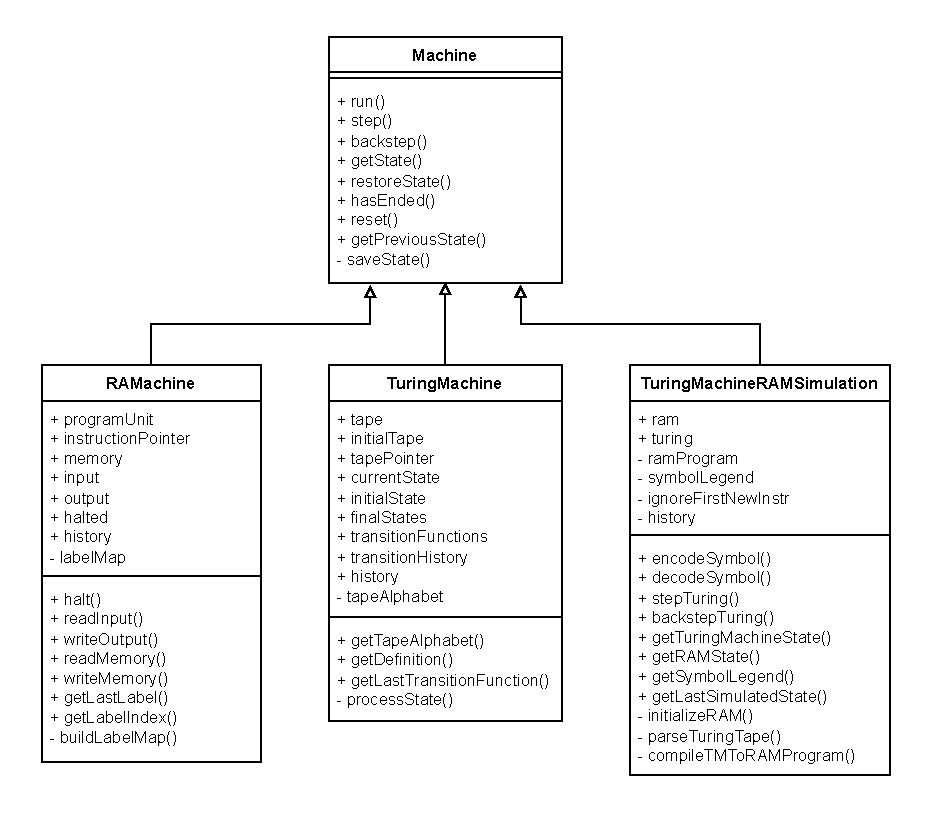
\includegraphics[width=0.72\textwidth]{Figures/class_diagram.pdf}
	\caption{Class diagram implementovaných strojů}
	\label{fig:class_machines}
\end{figure}

Turingův stroj je implementován s oboustranně nekonečnou pásku a vyžaduje u všech stavů předponou $q$.
Stroj také obsahuje mnoho kontrol parametrů před samotným definováním, 
nelze tedy například nadefinovat stroj, který obsahuje na pásce symboly mimo definovanou abecedu.

Pokud nastane v kterémkoli stroji chyba, dojde k vyvolání vlastní sjednocené chyby \texttt{MachineError}, 
která dědí ze zabudované třídy \texttt{Error}, takže ji lze odchytit shodně jako ostatní chyby přes \texttt{try/catch} syntaxi.
Třída obsahuje navíc informaci o tom, jaký stroj danou chybu vyhodil. 
To je výhoda například pro stroj simulace, kde pak můžeme zjistit přímo ve kterém konkrétním stroji chyba nastala.

Třída RAM stroje navíc obsahuje jednoduché rozhraní pro komunikaci s pamětí a páskou, díky kterému je pak požné definovat jednotlivé instrukce.
Všechny tyto instrukce implementují rozhraní \texttt{Instruction}. Příklad implementace jedné takové instrukce, \texttt{WriteOutput}, je zobrazen v kódě \ref{src:instructionExample}.
Každá instrukce má také parametr \texttt{options}, díky kterému můžeme přiřadit instrukci návěští nebo popisek, 
přes který lze nastavit různé \enquote{body synchronizace}, které se využívají například při simulaci, popsané v další sekci.

\begin{figure}[h!]
	\begin{lstlisting}[label=src:instructionExample,caption={Ukázka kódu instrukce \texttt{WriteOutput}}]
	class WriteOutput implements Instruction {
		options?: InstructionOption;
		private operandFrom: Operand;
		constructor(operandFrom: Operand, options?: InstructionOption) {
			this.operandFrom = operandFrom;
			this.options = options;
		}
		execute(machine: RAMachine): void {
			const value = resolveOperand(machine, this.operandFrom); // Operand muze byt konstanta nebo registr.
			machine.writeOutput(value); // Jedna z funkci rozhrani RAM stroje.
		}
		asComponent(): JSX.Element {
			return <span>WRITE({operandToJSX(this.operandFrom)})</span>; // Slouzi pro formatovany vypis dane instrukce.
		}
	}
	\end{lstlisting}
\end{figure}


\section{Průběh simulace}
Pro inicializaci stroje pro simulaci je nutné mít konkrétní instanci existujícího Turingova stroje.
Jednotlivé kroky inicializace jsou následující:
\begin{enumerate}
	\item Vytvoření slovníku podle postupu ze sekce \ref{sec:simulationTheory}.
	\item Kompilace kódu stroje RAM podle přechodových funkcí Turingova stroje. Jednotlivé kroky kompilace jsou následující:
	\begin{enumerate}
		\item Načtení vstupní pásky do paměti. Za poslední buňku se vloží číslo $-1$ pro ukončení načítání,
		\item inicializace řídících buněk paměti, sloužící pro běh simulace,
		\item překlad kódu podle algoritmu ze sekce \ref{sec:simulationTheory},
		\item výpis paměti na výstupní pásku.
	\end{enumerate}
	\item Dojde k enkódování Turingovy pásky podle již vytvořeného slovníku a její nahrání na vstupní pásku RAM stroje.
	\item Vytvoření instance samotného RAM stroje.
\end{enumerate}

Vstupní Turingův stroj může mít oboustranně nekonečnou pásku, ale simulovaný RAM stroj však simuluje pouze jednodstranně nekonečné pásky.
Kvůli tomu obsahuje RAM stroj navíc podmínky na ošetření, zda páskou nepřesahuje meze. 
Pokud ano, simulace se zastaví a stroj vyhodí příslušnou chybu. 

V paměti stroje RAM jsou první 3 buňky alokovány pro správu stroje a zbytek je určen pro obsah pásky. První buňky slouží při běhu simulace k následujícím účelům:
\begin{itemize}
	\item První buňka odkazuje na aktuální pozici na pásce,
	\item druhá slouží, během části rozřazování (z algoritmu v sekci \ref{sec:simulationTheory}), k uchování hodnoty aktuální buňky,
	\item třetí buňka není během simulace využita. Použita je pouze při výpisu výsledného stavu na výstupní pásku.
\end{itemize}

Ze vstupní pásky je monžé načíst libovolný počet $\square$ symbolů, 
avšak při výpisu nesmí být více než 2 prázdné znaky za sebou, tímto se výpis ukončí.
Běžně by se výspup ukončil již po prvním prázdném znaku, 
ale v tomto případě podpory prázdných znaků jej lze použít jako levé \enquote{zarážedlo} pásky.

\section{Uživatelské rozhraní}
Uživatelské rozhraní tvoří jedna responzivní stránka, která je rozdělena do dvou částí. V první části si uživatel zvolí stroj k simulaci 
a ve druhé částí již může daný stroj simulovat a sledovat jeho průběh. Vzhled stránky je vyzobrazen na obrázku \ref{fig:ui}.

\begin{figure}[h!]
	\centering
	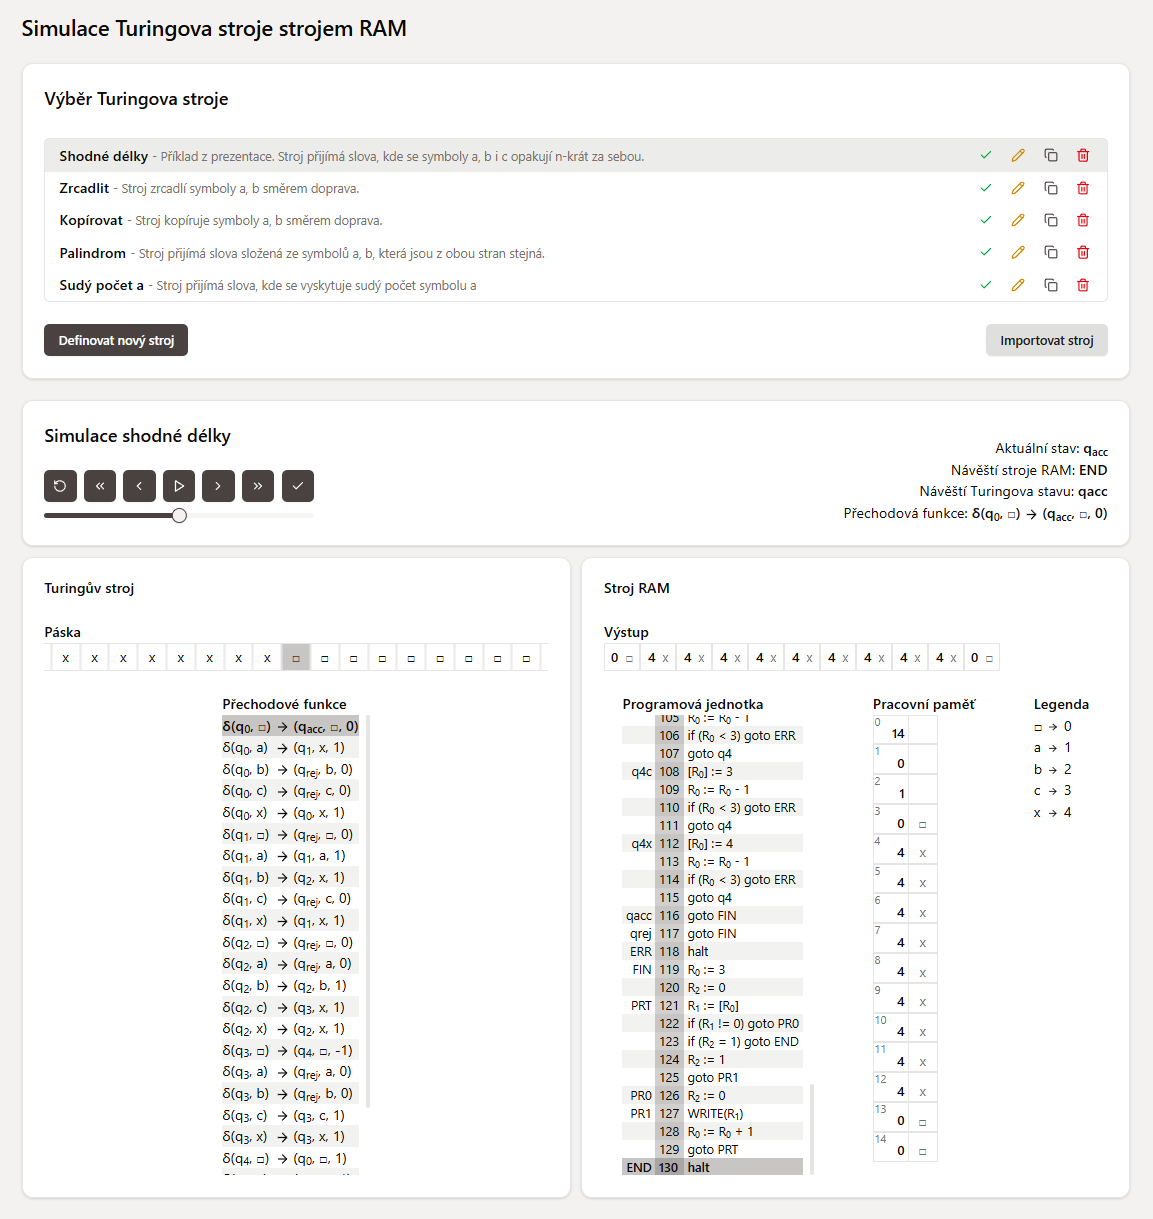
\includegraphics[width=1\textwidth]{Figures/ui.png}
	\caption{Uživatelské rozhraní aplikace}
	\label{fig:ui}
\end{figure}

První část také obsahuje možnost definice vlastního stroje či sdílení a import jiných strojů. 
Obě možnosti přidání strojů obsahují ošetření vůči nadefinování neplatného stroje.

Průběh simulace ve druhé části je možné krokovat buď podle jednoho kroku Turingova stroje, nebo podle kroku stroje RAM.
Dalšími možnostmi krokování jsou ekvivalentní kroky zpět, reset, konec a automatický běh, u kterého je možné si nastavit rychlost.
Tlačítko konce je limitováno na $2000$ kroků, aby se předešlo zacyklení běhu simulace. 
To je však možné obejít ručním krokováním nebo automatickým během simulace.

Vedle krokování jsou vypsány různé informace a stavy jednotlivých strojů, 
kdy po najetí na ně je zobrazen detailnější popis, co která hodnota znamená.

Část simulace Turingova stroje je sestavena z \textit{interaktivní pásky}, kde je aktuální pozice pásky vždy na středu a pásku je také možné
na chvíli myší nebo dotykem posunout a nahlédnout tak na momentálně skryté buňky. 
Další část obsahuje \textit{seznam přechodových funkcí} se zvýrazněnou aktuální funkcí, která zůstane vždy viditelná.

Část simulace RAM stroje obsahuje o poznání více prvků. Jako první je zobrazena \textit{vstupní} nebo \textit{výstupní páska}.
Výstupní páska je zobrazená pouze ve fázi zápisu na výstup, jinak je vždy zobrazena páska vstupní. 
Jednotivé buňky obou pásek obsahují také ekvivaltní znak odpovídající číslu po dekódování.
Dalším prvkem je \textit{programová jednotka}, která obsahuje seznam instrukcí, včetně návěští.
Shodně jako u přechodových funkcí Turingova stroje je i tady zvýrazněna aktuální instrukce, která zůstane vždy viditelná.
Další částí je \textit{pracovní paměť} stroje, kde je od 4. buňky také zobrazen ekvivalentní znak po dekódování.
Posledním prvek stroje RAM je \textit{legenda} (slovník).